% ---------------------------------------------------------------------------------
% Chapter: RA2
% $Id: RA2.tex,v 1.2 2012/02/04 22:54:40 matsch Exp $

\section{The RA2 analysis} \label{sec:RA2:RA2analysis}

\begin{figure}
  \begin{center}
    \begin{tabular}{ccc}
      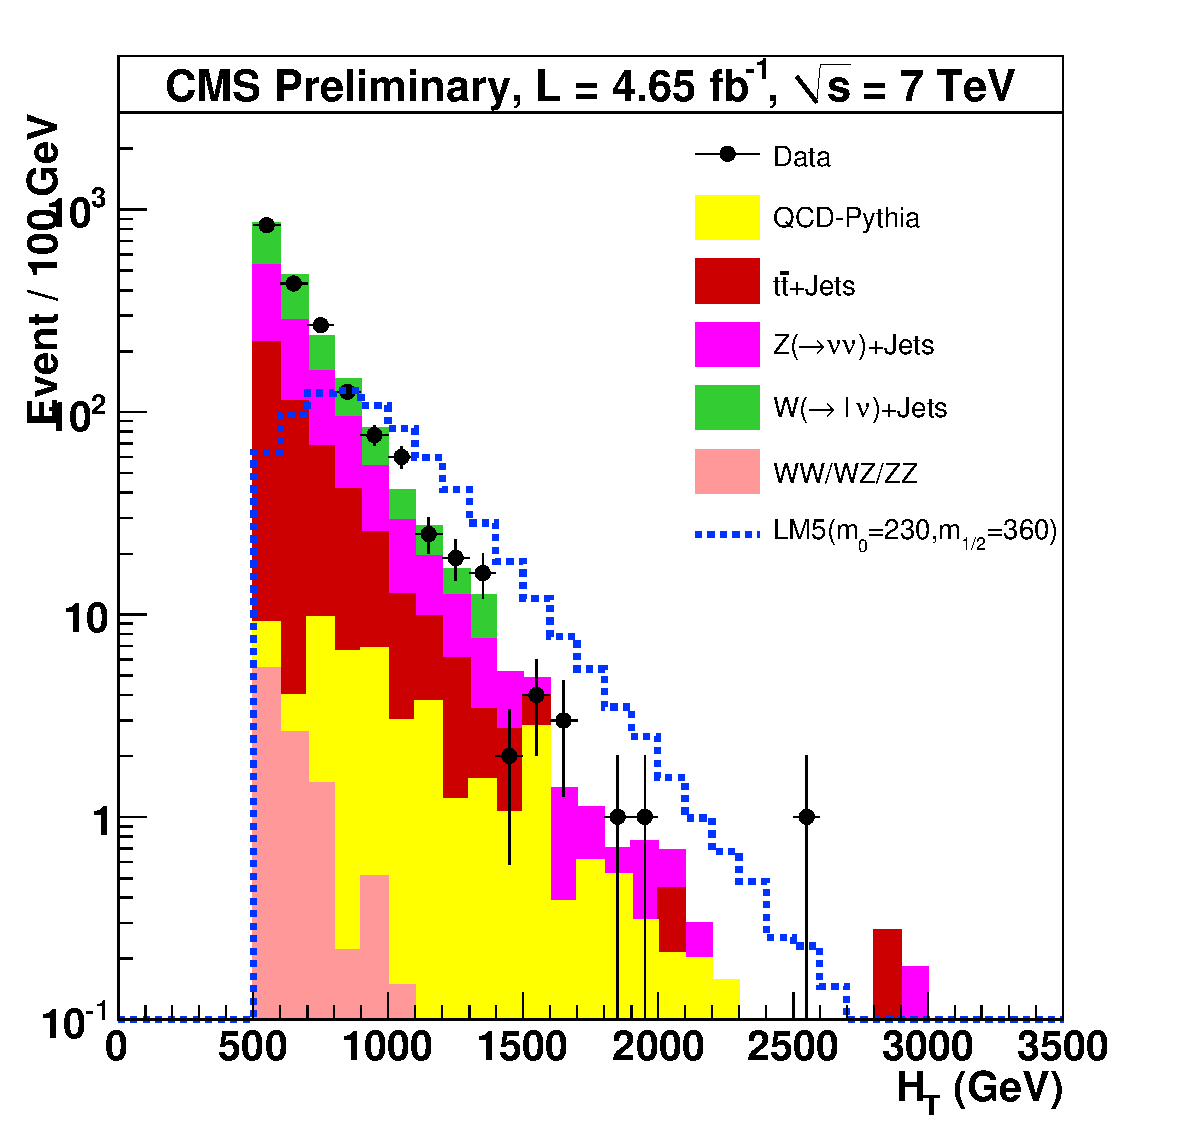
\includegraphics[width=0.5\textwidth]{figures/RA2/c_RA2_HTMHT_3J_dPhi_lepVeto_h_HT.pdf} &
      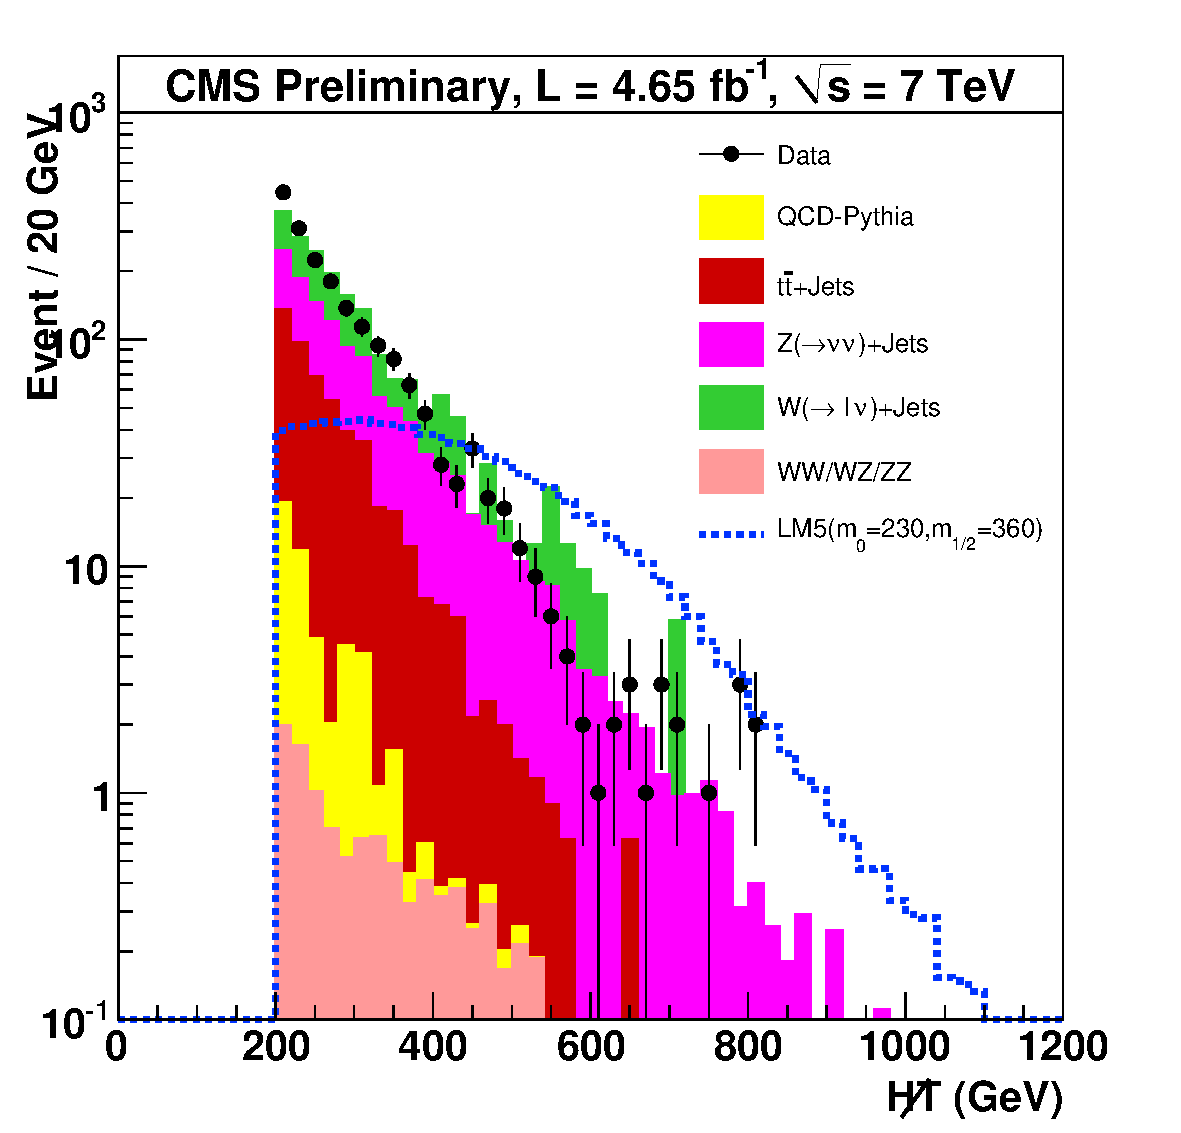
\includegraphics[width=0.5\textwidth]{figures/RA2/c_RA2_HTMHT_3J_dPhi_lepVeto_h_MHT.pdf} &
      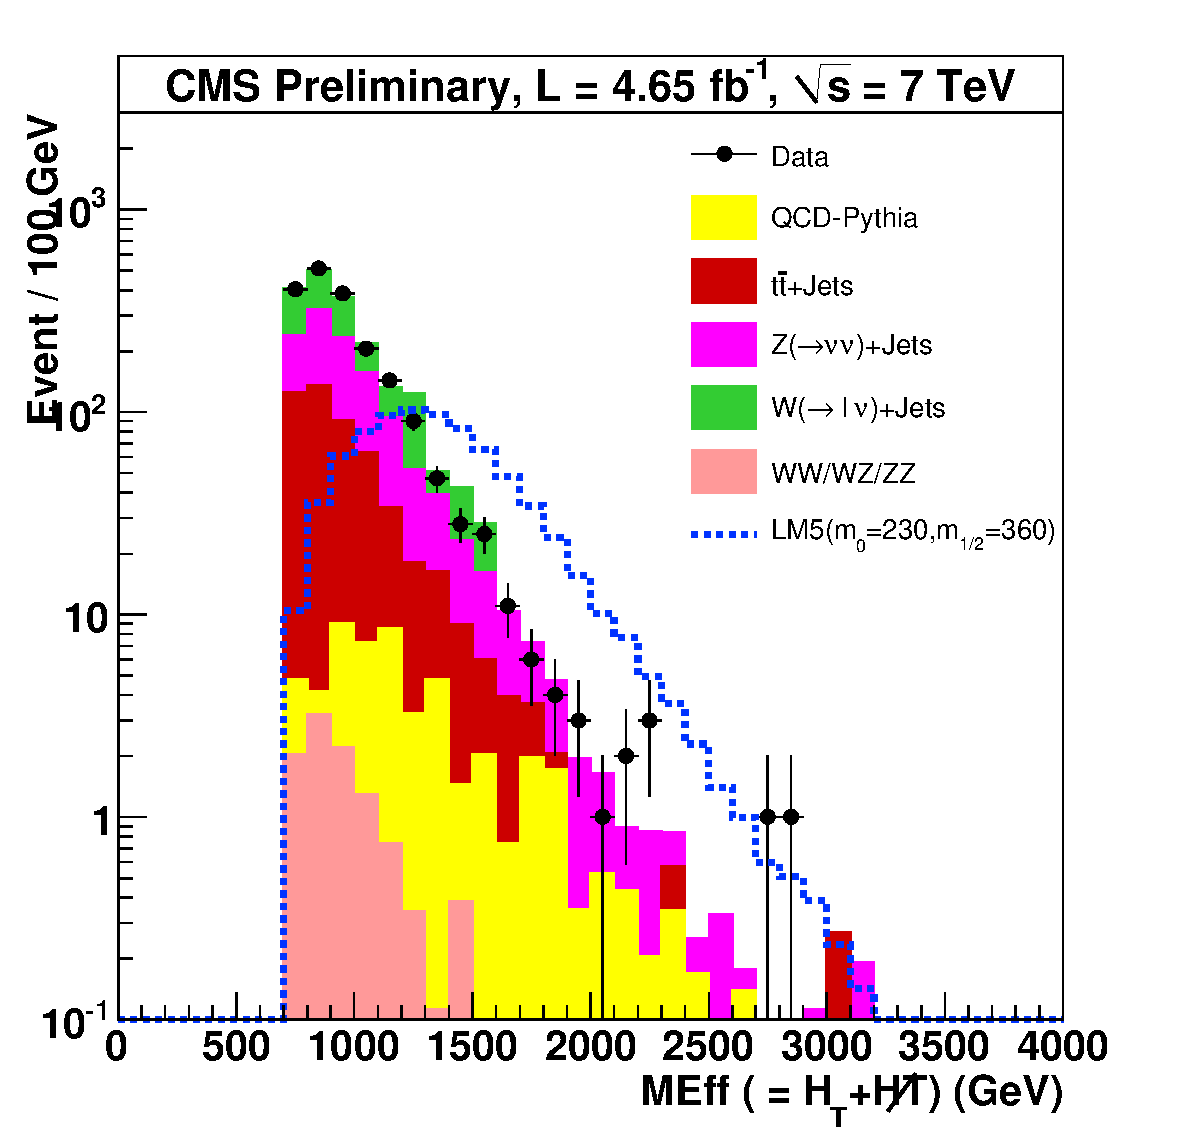
\includegraphics[width=0.5\textwidth]{figures/RA2/c_RA2_HTMHT_3J_dPhi_lepVeto_h_MEff.pdf} \\ 
    \end{tabular}
  \end{center}
  \caption{\todo{Add caption, point out difference to proper combination}}
  \label{fig:RA2:Results:Prediction}
\end{figure}




%%As outlined before in \qsec{sec:Theory:SUSY}, \susy is a promising and one of the most extensively studied frameworks for physics beyond the \sm.
%%Hence, \susy often serves as a guideline in the design of new-physics searches at collider experiments.
%%At the \lhc, sparticles can be produced, in particular squarks and gluinos via the strong interaction in the initial $pp$ collisions.
%%Due to their high masses, they subsequently decay in cascades into \sm particles with large momenta.
%%Again, since the sparticles are expected to be coloured, they will predominantly decay into coloured \sm particles and hence result in jets in the detector.
%%In case R-parity is conserved, the sparticles will be created in pairs and the LSP will be stable.
%%If only weakly interacting, such as the neutralino in the \mssm, the LSP will not produce any direct signal in the detector but will manifest as an imbalance in the observed total transverse momentum (\emph{missing transverse momentum} `\met') in the event.
%%
%%Since, of course, it is not known what kind of new physics --- if at all --- is realised at the \tevnospace scale, it is not clear either what kind of signature exactly to expect at the \lhc experiments.
%%The \cms \susy group therefore conducts a variety of searches for new physics covering a broad range of possible signatures which are motivated but not limited to supersymmetric models~\cite{bib:CMS:PhysicsResultsSUS}.
%%They can be roughly categorised as searches in lepton, photon, or multijet final states, each time accompanied by \met.
%%Each channel is covered by several analyses with different techniques and focus, thus allowing for mutual cross checks and lowering the model dependence.
%%
%%The multijet (\emph{all-hadronic}) final state is characterised by several high-\pt jets, large \met, and no isolated leptons.
%%Given the strong production mechanism and the consequent decay modes \addref, this channel has the largest branching ratio and can reach highest sensitivity.
%%At the same time however, it faces a huge background from \sm processes with the same signature, where \met is caused by neutrinos or instrumental effects.
%%%At the same time however, it faces a huge background from \sm processes with the same signature, such as \ZInvJets events as well as \ttbar and \WJets events, where the $W$ bosons either decay into light leptons which are not identified or into hadronically decaying \ltau leptons.
%%%In these cases, genuine \met is caused by neutrinos.
%%%A different major background arises from QCD multijet events where one or more jets are severely mismeasured because of leptonically decaying heavy-flavour hadrons inside the jet or because of instrumental effects.
%%
%%The presented analysis, in the following termed \emph{jets+met} analysis, has been designed as an inclusive search for new physics with minimal kinematic biases induced by the event selection in order to provide a high acceptance for a wide range of possible new physics scenarios with all-hadronic final states.
%%Therefore, the central observables in the analysis are \HT, the scalar sum of the jet transverse momenta, and \MHT, the missing transverse momentum computed from the jet momenta.
%%The broad acceptance requires a particularly precise understanding of the involved \sm backgrounds.
%%Hence, the essential feature of this analysis are robust methods to measure the full background spectra directly from data with minimal reliance on simulation.
%%The analysis has been initially published based on the 36\pbinv of data acquired by \cms in 2010~\cite{springerlink:10.1007/JHEP08(2011)155}.
%%This thesis focuses on an update which was performed with \lumiratwo from the 2011 data~\cite{CMS-PAS-SUS-11-004}.
%%
%%\cms has performed further searches in the all-hadronic channel complementing the \ratwo analysis~\cite{PhysRevLett.107.221804,bib:MT2_2011,CMS-PAS-SUS-11-008}.
%%These analyses are typically based on the assumption of initial pair-production of heavy particles and its implications.
%%Hence, different kinematic variables such as \alphat~\cite{PhysRevLett.101.221803}, $M_{\text{T},2}$~\cite{Lester:1999tx,Barr:2003rg}, or the `razor' variables $R$ and $M_{R}$~\cite{Rogan:2010kb} are exploited in order to reduce the \sm backgrounds, in particular QCD.
%%The ATLAS collaboration also published results from searches for new physics in similar all-hadronic final states\addref.
%%
%%This Chapter is organised as follows.
%%In \qsec{sec:RA2:EvtSel}, the selection of a general data set is described, from which later on more confined sets are defined in order to search for deviations from the expected \sm backgrounds.
%%The measurement of the latter from data is discussed in \qsec{sec:RA2:BkgEstimation}. 
%%Special emphasis is put on the QCD background, because the resolution measurements presented in \qsecs{sec:ResCore}{sec:ResTails} are an essential input.
%%Finally, in \qsec{sec:RA2:Results}, the results are interpreted.
%%
%%
%%(\todo{to introduction} Therefore, the investigated signatures in the search for new physics presented in this thesis have been motivated by the expectations from certain \susy scenarios.
%%However, it should be stressed, that the search has been designed in a most generic way and is sensitive to many possible realisations of physics beyond the \sm.)
%%
%%
%%
%%\section{Sample and Event Selection} \label{sec:RA2:EvtSel}
%%The presented analysis was performed on data from $pp$ collisions at a centre-of-mass energy of 7\tev which were acquired from March to June 2011 by the CMS experiment.
%%With all subdetectors fully functional, an integrated luminosity of \lumiratwo was recorded.
%%Events were collected by triggering on $\HT^{\text{trigger}}$ and, for most of the data, at the same time on $\MHT^{\text{trigger}}$, where $\HT^{\text{trigger}}$ and $\MHT^{\text{trigger}}$ are computed from calorimeter jets clustered with the iterative-cone algorithm with cone size $0.5$.
%%The efficiency of the combined set of triggers has been measured in data using a more inclusive  $\HT^{\text{trigger}}$ trigger as a function of the offline \HT and \MHT defined below in \qsec{}:
%%it is greater than $99\%$ for \mbox{$\HT > 350\gev$} and \mbox{$\MHT > 200\gev$}~\cite{CMS-PAS-SUS-11-004}.
%%
%%All offline physics objects have been reconstructed with the \emph{particle-flow} (`\PF') algorithm~\cite{CMS-PAS-PFT-09-001,CMS-PAS-PFT-10-002}.
%%For this procedure, the information from all CMS subdetectors are combined to identify different types of particles, such as charged or neutral hadrons, photons, muons, and electrons.
%%From these particles, jets are clustered using the \antikt jet algorithm~\cite{1126-6708-2008-04-063} with a distance parameter \mbox{$R=0.5$}.
%%Their momenta are corrected on average by removing the $\eta$ and \pt dependence as well as by compensating for the impact of additional pile-up interactions to those which would have been obtained if all particles were perfectly measured.
%%The calibration constants were derived from simulation.
%%%They are corrected with calibration constants derived from simulation in order to remove the $\eta$ and \pt dependence of their energy scale as well as to compensate for the impact of additional pile-up interactions.
%%Residual small response differences between data and simulation are corrected by applying additional calibration constants to the data, which are measured from photon+jets and dijet data~\cite{1748-0221-6-11-P11002}.
%%\todo{Explain this in more detail in the jet section.}
%%
%%Several \emph{filters} have been employed in order to identify events where the object reconstruction failed or was spoiled by instrumental effects or which originated in beam-background processes.
%%In rare cases, these events feature large \MHT and can populate the search regions.
%%Although their absolute contribution is small \todo{put some number}, they might substantially falsify the analysis result due to the likewise tiny expected rate of signal processes.
%%Therefore, these events are not used in the further analysis.
%%\addfig{effect of cleaning (note by Colin, new 2011 results)}
%%
%%Particles originating from displaced vertices in satellite collisions as well as from beam-related processes such as muons from proton collisions outside the detector (\emph{beam halo}) possibly prevent a proper event reconstruction.
%%Therefore, each event is required to have at least one high-quality primary vertex which has been determined from more than four tracks and is located within $24\cm$ in $z$ and $2\cm$ in $xy$ direction from the nominal interaction point.
%%Furthermore, the \emph{Cathode Strip Chamber} subdetector is utilised to identify and reject events with muons traversing parallel to the beam and hence likely stem from a beam halo~\cite{CMS-PAS-MUO-10-002}.
%%
%%In some events, anomalous signals in the electromagnetic or hadronic calorimeters are caused by particles hitting the readout electronics, scintillation fibres, or photomultipliers.
%%Dedicated criteria have been defined to identify and reject these events~\cite{CMS-PAS-EGM-10-006,CMS-DP-2010-025}.
%%Faked large energy deposits are in rare cases also produced by electronic noise in the ECAL readout system at random times and can overlap with a collision event.
%%These anomalies can be identified and in fact removed using timing and pulse-shape information, thus allowing further usage of the event~\cite{CMS-PAS-JME-10-009}.
%%%Additional rare noise has been identified to affect the ECAL endcaps coherently with the muons systems.
%%%It has been suppressed by selecting events with less than $2\,500$ energy deposits in the endcaps (\emph{EE noise filter}).
%%
%%Reliable track reconstruction is ensured by requiring the fraction of tracks passing high-quality criteria to be greater than $25\%$, if there are at least ten tracks in the event.
%%In addition, the scalar sum of the \pt of tracks associated to the primary vertex has been required to be less than $10\%$ of the scalar sum of jet \pt of all jets within the tracker acceptance in order to ensure.
%%Moreover, events with seriously misreconstructed muons are rejected~\cite{springerlink:10.1007/JHEP08(2011)155,CMS-PAS-SUS-11-004}.
%%
%%About $1\%$ of the crystals of the electromagnetic calorimeter are not read out because of malfunctioning on-detector electronics.
%%If energy is deposited in these crystals, it is lost in the object reconstruction.
%%The affected events are identified and rejected either by the information from a parallel readout chain of the trigger system or, in case it is not available, by measuring the amount of energy deposited in the crystals surrounding the affected regions~\cite{CMS-PAS-JME-10-009}.
%%
%%After the trigger and filter requirements, the full event selection is defined as follows in two succesive steps starting with the (\emph{baseline selection}):
%%\begin{itemize}
%%\item There are at least three jets with \mbox{$\pt > 50\gev$} and $|\eta| < 2.5$ in order to select events with a multijet final state topology.
%%\item A high energy scale of the hard-scattering process is ensured by requiring \mbox{$\HT > 350\gev$}, where
%%  \begin{equation*}
%%    \HT \equiv \sum_{i} \pti{i}
%%  \end{equation*}
%%  and $i$ runs through all jets with \mbox{$\pt > 50\gev$} and \mbox{$|\eta| < 2.5$}.
%%\item In order to suppress QCD contributions, \mbox{$\MHT > 200\gev$} has to be met, where
%%  \begin{equation*}
%%    \MHT \equiv -\left|\sum_{i} \ptivec{i} \right|
%%  \end{equation*}
%%  and $i$ runs through all jets with \mbox{$\pt > 30\gev$} and \mbox{$|\eta| < 5$} \todo{motivate choice of different jets in \HT and \MHT}.
%%\item Remaining QCD events in which large \MHT is caused by a single mismeasured jet are vetoed by requiring \mbox{$\Delta\phi(\ptivec{i},\MHTvec) > 0.5$}, \mbox{$i\in{1,2}$}, and \mbox{$\Delta\phi(\ptivec{3},\MHTvec) > 0.3$}, \ie \MHT must not be aligned with the transverse momenta of one of the leading three jets.
%%\item \ttbar and \WJets events with leptons in the final state are suppressed by rejecting events containing isolated muons or electrons with \mbox{$\pt > 10\gev$} and \mbox{$|\eta| < 2.4$} or \mbox{$|\eta| < 2.5$}, respectively~\cite{CMS-PAS-SUS-11-004}.
%%\end{itemize}
%%Three \emph{search regions} are defined by tighter criteria on \HT and \MHT \wrt the baseline selection.
%%They are selected based on the amount of \sm background and the expected signal efficiency for the \cmssm:
%%\begin{itemize}
%%\item The \emph{medium search region} requires \mbox{$\HT > 500$} and \mbox{$\MHT > 350\gev$}.
%%\item The \emph{high-\HT search region} requires \mbox{$\HT > 800\gev$}.
%%This selection is in particular sensitive to events with high multiplicities as in case of long cascade decays where most of the energy is distributed to the strongly interacting particles.
%%\item The \emph{high-\MHT search region} requires \mbox{$\MHT > 500\gev$} in order to improve the rejection of \sm backgrounds, especially QCD.
%%\end{itemize}
%%The expected total event yields\footnote{The simulated yields for the individual background contributions are quoted in Tab.~1 in~\cite{CMS-PAS-SUS-11-004}.} from the \sm background processes as obtained from simulation after the baseline and three search selections are listed in \qtab{tab:RA2:EventSel:EventYields}.
%%They are compared to the expectations for a specific \susy model.
%%\begin{table}[!htb]
%%  \begin{center}
%%    \caption{Number of events expected from the \sm background processes in \lumiratwo after the baseline and search selections as predicted by simulation.
%%      The contributions have been obtained using the \pythia generator in case of QCD and the \madgraph generator otherwise.
%%      For comparison, the expected number of signal events for the \cmssm parameter point `LM4', defined by \mbox{$m_{0} = 210\gev$}, \mbox{$m_{1/2} = 285\gev$}, \mbox{$A_{0} = 0$}, \mbox{$\tan\beta = 10$}, and \mbox{$\mu > 0$}, is given to illustrate the impact from possible new physics.
%%      The events have been generated using \pythia assuming a next-to-leading order LM4 signal cross section of \mbox{$2.5\;\text{pb}$}, which has been computed using the \prospino programme~\cite{Beenakker:1996ed}.
%%    }
%%    \label{tab:RA2:EventSel:EventYields}
%%    \begin{tabular}{l r@{.}l r@{.}l r@{.}l r@{.}l}
%%      \toprule
%%      & \multicolumn{2}{c}{Baseline} & \multicolumn{2}{c}{Medium} & \multicolumn{2}{c}{High-\HT} & \multicolumn{2}{c}{High-\MHT} \\
%%      & \multicolumn{2}{c}{(\HT$>$350~\gev)}  & \multicolumn{2}{c}{(\HT$>$500~\gev)} & \multicolumn{2}{c}{(\HT$>$800~\gev)}  & \multicolumn{2}{c}{(\HT$>$800~\gev)}  \\
%%      & \multicolumn{2}{c}{(\MHT$>$200~\gev)} & \multicolumn{2}{c}{(\MHT$>$350~\gev)} & \multicolumn{2}{c}{(\MHT$>$200~\gev)} & \multicolumn{2}{c}{(\MHT$>$500~\gev)} \\
%%      \midrule
%%      \sm
%%      & 987&0 
%%      &  95&0 
%%      &  83&0 
%%      &   7&5  \\
%%      \midrule
%%      LM4
%%      & 742&0 
%%      & 318&0 
%%      & 304&0 
%%      &  54&0  \\
%%      \bottomrule
%%    \end{tabular}
%%  \end{center}
%%\end{table}
%%
%%
%%
%%\section{Estimation of the Standard Model Backgrounds From Data} \label{sec:RA2:BkgEstimation}
%%Several \sm processes with genuine \met caused by neutrinos constitute backgrounds to the selected signal samples.
%%These are \ZInvJets events as well as \ttbar and \WJets events, where the $W$ bosons either decay into light leptons which are not identified or into hadronically decaying \ltau leptons.
%%A different major background arises from QCD multijet events where one or more jets are severely mismeasured because of leptonically decaying heavy-flavour hadrons inside the jet or because of instrumental effects.
%%The expected, full \HT and \MHT spectra of the \sm background processes are modelled from data, as discussed below, thus avoiding dependence on the simulation.
%%
%%
%%
%%\subsection{Non-QCD Backgrounds}
%%% --- Z to inv bkg ------------------------------------
%%Events with jets and a \Z boson produced in association which subsequently decays into two neutrinos form an irreducible \sm background in the selected data sample.
%%
%%Its contribution can be estimated from data in a straightforward way using \mbox{$Z\rightarrow e^{+}e^{-}$}+jets or \mbox{$Z\rightarrow \mu^{+}\mu^{-}$}+jets events and ignoring the leptons in the reconstruction in order to mimic the neutrino-induced \MHT in \ZInvJets events.
%%After corrections for the acceptance, efficiency, and different branching ratios, their topology is directly reproduced due to the lepton-universality of the weak interaction and the expected background yield is obtained by applying the jet-related selection criteria.
%%However, given the low yield of the \mbox{$Z\rightarrow ll$}+jets events, this method is used as a cross-check verifying the results of the primary method.
%%
%%As primary method, the kinematic properties of \ZInvJets events are predicted from a control sample of $\gamma$+jets events.
%%The structure of the production process is the same for the neutral electro-weak bosons at \pt larger than the \Z mass with asymptotically vanishing mass effects and the cross-section ratio depends mostly on the different size of the electro-weak couplings.
%%In order to obtain a reliable background prediction, contributions to the control sample from QCD multijet events where a photon originates not in the hard scattering process but in fragmentation inside jets or neutral pion decays are minimised by imposing tight isolation criteria on the reconstructed photons.
%%The residual contamination is estimated from NLO \textsc{Jetphox} calculations and data, respectively~\cite{PhysRevD.73.094007,PhysRevLett.106.082001,PhysRevD.84.052011}\todo{verify}.
%%The selection requirements have also been found to sufficiently suppress contamination of the control sample by possible signal events.
%%Then, the background prediction is obtained by removing the $\gamma$ in the event reconstruction, applying the jet-related selection requirements to the control sample, and finally scaling the resulting number of $\gamma$+jets events to account for the differences in branching ratios as well as acceptance and reconstruction efficiencies, which are determined from a \madgraph simulation~\cite{Alwall:2007st}.
%%The dominant uncertainties of the method are an uncertainty of $12\%$ on this phenomenological scale factor as well the statistical uncertainty of about $15\%$ due to the size of the control sample.
%%
%%
%%% --- Lost-lepton and hadronic tau bkg ---------------------------------
%%Events from \ttbar and \WJets production can fake the signal topology if the $W$ bosons decay into leptons and neutrinos thus inducing \met.
%%They are not rejected by the event selection either in case of a hadronically decaying \ltau lepton (\emph{hadronic-$\tau$}) or in case the veto of a light lepton fails (\emph{lost-lepton}) because it is out of geometric or kinematic acceptance, is not identified, or not isolated.
%%Both components are predicted using a $\mu$+jets control sample.
%%
%%In case of the \lostlep background, control samples for the different search regions are selected by applying the full event selection but without the explicit lepton veto.
%%Instead, exactly one well-identified and well-isolated muon is required.
%%Moreover, only events with a \emph{transverse mass} \mbox{$m_{\text{T}}\equiv\sqrt{2\pt(\mu)\met(1-\cos(\Delta\phi))}$} of less than 100\gev are selected, with $\Delta\phi$ being the difference in azimuthal angle between the muon and the \met vector, which enhances the \ttbar and \WJets contributions in the sample and sufficiently suppresses the presence of possible signal events.
%%The \lostlep contribution in the search regions is modelled by weighting the number of events in the control sample according to the lepton identification and isolation efficiencies as well as acceptance factors.
%%The identification and isolation efficiencies are measured separately for electrons and muons from $Z$+jets data as a function of lepton \pt using a tag-and-probe method.
%%They are parametrised by the angular distance between the lepton and the nearest jet as well as the lepton $\eta$, respectively, in order to take into account kinematic differences of the $Z$+jets events.
%%Residual kinematic differences have been studied using simulated events and have been found to result in an underprediction of the background of about $7\%$, for which the final prediction has been corrected.
%%The acceptance factor is determined from simulated \ttbar and \WJets events.
%%Besides the correction of the kinematic bias, the dominant uncertainty of the prediction arises from the statistical uncertainty of $22\%$ due to the size of the $\mu$+jets and $Z$+jets control samples.
%%
%%In case of the \hadtau background, the control sample is selected using a single-muon trigger and requiring exactly one muon with \mbox{$\pt > 20\gev$} and \mbox{$|\eta| < 2.1$}.
%%Again, the transverse mass requirement is imposed to prevent signal contamination of the control sample.
%%Due to the lepton universality of the weak interaction, the hadronic part of the events in the control sample correspond to the non-$\tau$ part of the \hadtau background events.
%%Hence, the muon is used to model the $\tau$ jet by scaling its transverse momentum with a factor sampled from a template of the visible $\tau$-\pt fraction, which has been obtained from simulated events.
%%After recomputation of \HT and \MHT, where the additional jet is taken into account, the \hadtau contribution in the search region is predicted by applying the search selection to the modified control sample and scaling the event yield by the branching fraction of $W$ bosons decaying into hadronically decaying $\tau$ leptons and into muons.
%%Corrections are applied to take into account the muon geometric and kinematic acceptance, which is derived from simulation, as well as the identification and isolation efficiencies, which are measured from $Z$+jets data as in case of the \lostlep background.
%%The dominant uncertainties of the prediction are the uncertainty on the $\tau$-\pt template and the statistical uncertainty due to the size of the control sample, each amounting to about $3\%$.
%%
%%
%%\subsection{QCD Background}
%%\todo{discuss jet response, mc scaling} \\
%%\todo{discussion: where does qcd contribute (high ht search region, i.e. high m1/2)}
%%
%%Modelling of the QCD multijet background is challenging because the underlying QCD production processes are theoretically difficult to compute and the simulation of jet measurements requires a particularly precise understanding of the detector components and effects. 
%%In QCD multijet events, \MHT arises from mismeasurements due to the jet-\pt response \alreadydefined{response}.
%%While the almost Gaussian core of the response distribution around unity is inherent to the principle of energy and momentum measurement of a detector, the tails of extremely low response originate both in heavy-flavour hadrons inside jets which decay into among others neutrinos and in instrumental effects such as punch-through of energetic particles as well as masked detector regions.
%%\todo{add study here or elsewhere of response components (Sue Ann)}
%%Although the tail component contributes only below the percentage level to the total distribution, it leads to severe jet-\pt mismeasurements resulting in possibly large values of \MHT and thus promoting an event into the search regions.
%%
%%\subsubsection{Description of the Rebalance-And-Smear Method}
%%The QCD background is estimated from inclusive multijet data using a simplified simulation obtained by a \emph{rebalance-and-smear} (`R+S') method~\cite{bib:phd:sueann,CMS-PAS-SUS-11-004,springerlink:10.1007/JHEP08(2011)155}.
%%An estimator of \MHT is obtained by first rebalancing the jet momenta in each event, taking into account the jet-\pt resolution, and then weighting the rebalanced momenta by the full jet-\pt response distribution in order to predict the complete multijet kinematics.
%%
%%In the rebalance step, a sample of \emph{seed events} is created from multijet data.
%%The measured jet momenta are adjusted, resulting in \emph{seed jets}, to regain approximate transverse momentum balance as expected for QCD events at particle-jet level.
%%Technically, this is achieved with a kinematic fit~\addref.
%%\pt, $\eta$, and $\phi$ of the jets are varied in order to find a configuration which obeys the transverse momentum balance constraint and minimises the residuals of measured and modified jets.
%%The measurement uncertainties are approximated by the Gaussian core component of the jet-\pt response distribution since the rebalance procedure is insensitive to the tiny non-Gaussian tails.
%%Only jets with \mbox{$\pt > 10\gev$} are used in order to reduce the impact of pile-up interactions, which produce a large number of low-\pt jets not originating in the considered hard interaction and thus spoiling the momentum balance constraint.
%%Possible biases introduced by this requirement have been observed to affect the final prediction by less than $10\%$ and are considered in the uncertainties.
%%Importantly, contributions to the seed sample from the \ttbar or electro-weak backgrounds as well as possible signal processes are negligible since also these events will be transformed into QCD-like events with balanced transverse momenta and their cross section is smaller by orders of magnitude than the QCD-multijet cross-section.
%%
%%In the smear step, the four-momentum of each seed jet is scaled by a random factor generated from the full jet-\pt response distribution, thus modelling effects of the measurement and resulting in the expected detector-level jet.
%%The kinematic of the original QCD events is preserved in the obtained sample of events with smeared jets.
%%Hence, the expected distributions of \HT and \MHT as well as other jet-related variables are predicted after applying the full analysis event selection.
%%In order to improve the statistical precision of the prediction, the smear step of the procedure is repeated 1000 times for each seed event.
%%Biases due to the correlated seeds are avoided by incorporation of a bootstrap technique~\cite{bib:bootstrap} when computing the mean and variance of the prediction.
%%
%%The performance of the R+S method has been studied using a sample of events simulated with \pythia.
%%The predicted \HT and \MHT distributions after a modified baseline selection, where the \HT and \MHT requirement has been dropped, respectively, are shown in \qfig{fig:RA2:SMBkg:RSClosure}.
%%They are compared to the distributions from the fully simulated events.
%%There is good agreement of the R+S prediction to the full simulation in the important medium-to-high \MHT region, except for the highest bin where the number of events are seriously overpredicted; the precise amount is difficult to quanitfy, however, since the statistical uncertaintiy of the expectation from the full simulation is large.
%%In the low \MHT region, the prediction fluctuates around the expectation by up to $20\%$, which is not covered by the statistical uncertainties.
%%The ratio of the predicted number of events to the number obtained with the full simulation for the different search selections is applied as a bias correction factor to the final prediction.
%%It is below $25\%$ in all cases.
%%The dominating biases of the method arise from the finite jet-\pt response parametrisation, the jet-\pt threshold of 10\gev for the rebalance step, and from migration effects due to the steeply falling jet-\pt spectrum in combination with the finite resolution.
%%\begin{figure}
%%  \begin{center}
%%    \begin{tabular}{cc}
%%%      \includegraphics[width=0.5\textwidth]{figures/ra2/} &
%%      & \includegraphics[width=0.5\textwidth]{figures/ra2/QCD_SmearingClosure_OnMC_LowHT_MHT.pdf} \\
%%    \end{tabular}
%%  \end{center}
%%  \caption{\fixme{Add HT distribution} Consistency test of the R+S method with \pythia-simulated events~\cite{CMS-PAS-SUS-11-004}: \HT (\textit{left}) and \MHT (\textit{right}) distributions predicted by the R+S method (circles) compared to the results of the full simulation (squares).
%%  }
%%  \label{fig:RA2:SMBkg:RSClosure}
%%\end{figure}
%%
%%
%%
%%\subsubsection{Jet Response Functions}
%%The jet-\pt response distributions are crucial input to the R+S method.
%%They are determined as described in \qsec{sec:Jets:Resolution:MCTruth} from a sample of QCD multijet events simulated with the \pythia event generator~\cite{Sjostrand:2006za}: to each of the two leading \todo{define leading at first appearance} generator-level jets the reco-level jet closest in \mbox{$\eta\times\phi$} is matched, and the response is computed as \mbox{$\ptreco / \ptgen$}.
%%The simulated distributions are adjusted to match the data as discussed in detail in \qsec{}.
%%In order to account for the dependence of the response on the energy of the jet as well as the different detector region, a set of response distributions for different bins of \pt and $|\eta|$ is compiled.
%%
%%
%%\subsubsection{Prediction of the QCD Background}
%%In contrast to the search sample, the multijet data input to the R+S method has been collected by triggering on $\HT^{\text{trigger}}$ only with no additional requirement on \MHT, which would bias the seed sample.
%%However, the lowest un-prescaled \HT trigger has a threshold of 500\gev.
%%Since the baseline selection requires \mbox{$\HT > 350\gev$} and since in course of the R+S procedure events can migrate in \HT, additional, prescaled trigger paths with thresholds down to 150\gev are utilised.
%%The data sample recorded by the different trigger paths are combined taking into account the prescales, which results in an increase of the statistical uncertainty of the prediction of about \todo{add number} because of single events with large weights.
%%Furthermore, to reduce the amount of processed data, only events containing at least two jets with \mbox{$\pt > 50\gev$} are considered for the seed sample.
%%The results of the R+S prediction in the different search regions are listed in \qtab{tab:RA2:Bkg:RS}.
%%\begin{table}[!htb]  
%%  \begin{center}
%%    \caption{\todo{Add caption}}\label{tab:RA2:Bkg:RS}
%%    \begin{tabular}{lllll}
%%      \toprule
%%      & Baseline & Medium & High-\HT & High-\MHT \\
%%      \midrule
%%      Bias-corrected prediction & 31.0 & 1.3 & 13.5 & 0.09 \\
%%      Total uncertainty ($\%$) & $^{+125}_{-116}$ & $^{+112}_{-107}$ & $^{+62}_{-44}$ & $^{+347}_{-345}$ \\
%%      \midrule
%%      Seed sample size ($\%$) & $\pm114$ & $\pm102$ & $\pm30$ & $\pm340$ \\
%%      Resolution core ($\%$) & $^{+10}_{-8}$ & $^{+3}_{-8}$ & $^{+9}_{-9}$ & $^{+1}_{-18}$\\
%%      Resolution tail ($\%$) & $^{+31}_{-19}$ & $^{+17}_{-34}$ & $^{+33}_{-31}$ & $^{+41}_{-36}$\\
%%      Flavour trend ($\%$) & $\pm10$ & $\pm10$ & $\pm10$ & $\pm10$\\
%%      R+S non-closure ($\%$) & $\pm40$ & $\pm40$ & $\pm40$ & $\pm40$\\
%%      Pile-up effects ($\%$) & $\pm10$ & $\pm10$ & $\pm10$ & $\pm10$\\
%%      \bottomrule
%%    \end{tabular}
%%  \end{center}
%%\end{table}
%%
%%
%%\subsubsection{Systematic Uncertainties}
%%Various sources of systematic uncertainties of the R+S method have been investigated.
%%Their impact on the prediction is also listed in~\qtab{tab:RA2:Bkg:RS}.
%%
%%As discussed above, the combined impact of the R+S biases has been found to affect the prediction by less than $25\%$ depending on the search region.
%%The final prediction is corrected for this bias and a conservative systematic uncertainty of $40\%$ is assigned.
%%
%%Furthermore, the uncertainties on the jet-\pt response measurements~\qsec{} are propagated to the prediction by repeating the R+S method with the response input changed by \mbox{$\pm1\sigma$}, leading to variations of the result of up to $40\%$.
%%
%%The simulated response distributions were derived using the \pythia event generator.
%%Variations of the R+S prediction due to the assumed flavour composition of jets were observed to be within $10\%$ when comparing to the results obtained with response distributions from the \madgraph generator~\cite{bib:phd:sueann,CMS-PAS-SUS-11-004,springerlink:10.1007/JHEP08(2011)155}.
%%
%%Residual effects from pile-up interactions have been investigated using a sample of simulated events, where the pile-up scenario has been reweighted to match the distribution expected for data from the machine conditions and the minimum-bias cross section.
%%No significant variations in the R+S prediction are present when shifting the mean of the pile-up distribution by \mbox{$\pm1$}.
%%Nonetheless, given the sizable statistical uncertainties of the different results, a conservative uncertainty of $10\%$ is assigned.
%%
%%
%%
%%\section{Results and Interpretation} \label{sec:RA2:Results}
%%The \HT and \MHT distributions in \lumiratwo of data after the baseline selection are shown in \qfig{fig:RA2:Results:HTMHT}.
%%They are compared to the expected \sm background contributions predicted using the data-driven methods described above.
%%\begin{figure}
%%  \begin{center}
%%    \begin{tabular}{cc}
%%      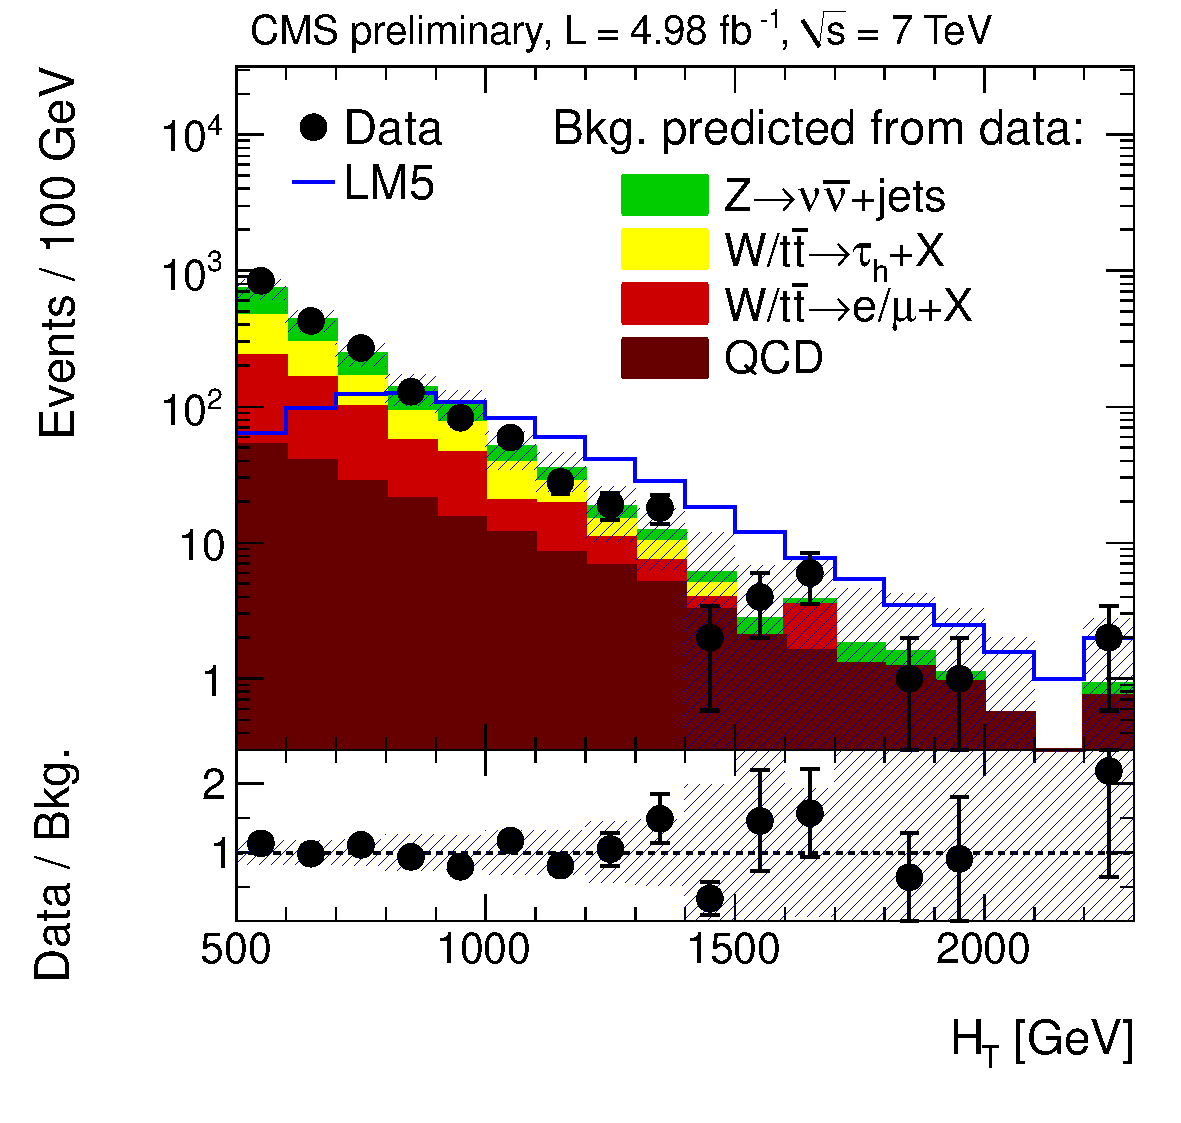
\includegraphics[width=0.5\textwidth]{figures/ra2/RA2DataVsEstimatedBkg_HT.pdf} &
%%      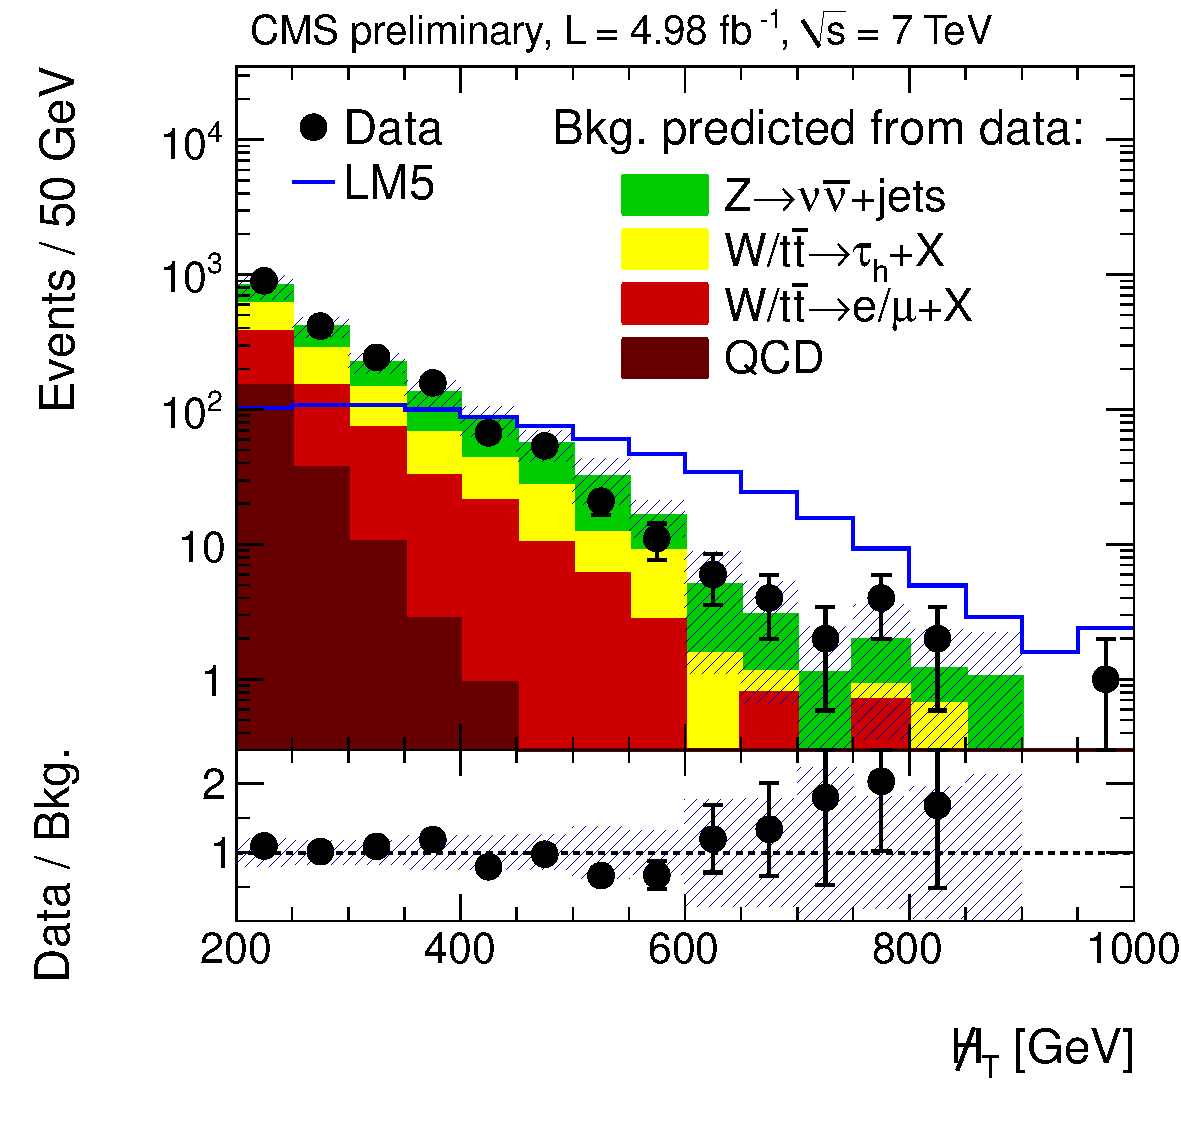
\includegraphics[width=0.5\textwidth]{figures/ra2/RA2DataVsEstimatedBkg_MHT.pdf} \\
%%    \end{tabular}
%%  \end{center}
%%  \caption{\todo{Add caption, point out difference to proper combination}}
%%  \label{fig:RA2:Results:HTMHT}
%%\end{figure}
%%
%%The number of events observed in data after the baseline and the different search selections is listed in \qtab{tab:RA2:Results:EventYields}.
%%It is compared to the yields expected from the different \sm background processes.
%%Although the data-driven methods allow for a prediction differential in \HT and \MHT, here integrated yields in the more inclusive search regions are considered in order to achieve maximal statistical precision.
%%A combined background expectation is derived by numerical convolution of the different probability density functions assigned to each uncertainty source of the individual background contributions, thus taking into account possible correlations between the estimation methods.
%%Following the Central Limit Theorem, the resulting probability density distribution is fitted with a Gaussian function, whose mean and standard deviation are listed as total expected background yield and its uncertainty, respectively.
%%It is below the \sm expectation obtained from simulation listed in \qtab{tab:RA2:EventSel:EventYields}, which emphasises the importance of simulation-independent, data-driven methods.
%%The observed number of events is compatible with the \sm expectation in all search regions.
%%\begin{table}[!htb]
%%  \begin{center}
%%    \caption{Expected event yields with statistical and systematic uncertainties, respectively, from the different \sm background processes in \lumiratwo as predicted by the data-driven methods after the baseline and search selections.
%%      The total background estimate is calculated as described in the text as mean of a Gaussian fit to the combined probability density of the various uncertainty contributions.
%%      It is compared to the observed number of events in data.
%%    }
%%    \label{tab:RA2:Results:EventYields}
%%    \begin{tabular}{l
%% r@{.}l@{$\;\pm\,$}r@{.}l@{$\;^{+}_{-}$}l
%% r@{.}l@{$\;\pm\,$}r@{.}l@{$\;^{+}_{-}$}l
%% r@{.}l@{$\;\pm\,$}r@{.}l@{$\;^{+}_{-}$}l
%% r@{.}l@{$\;\pm\,$}r@{.}l@{$\;^{+}_{-}$}l
%%}
%%      \toprule
%%      & \multicolumn{5}{c}{Baseline} & \multicolumn{5}{c}{Medium} & \multicolumn{5}{c}{High-\HT} & \multicolumn{5}{c}{High-\MHT} \\
%%      & \multicolumn{5}{c}{(\HT$>$350~\gev)}  & \multicolumn{5}{c}{(\HT$>$500~\gev)} & \multicolumn{5}{c}{(\HT$>$800~\gev)}  & \multicolumn{5}{c}{(\HT$>$800~\gev)}  \\
%%      & \multicolumn{5}{c}{(\MHT$>$200~\gev)} & \multicolumn{5}{c}{(\MHT$>$350~\gev)} & \multicolumn{5}{c}{(\MHT$>$200~\gev)} & \multicolumn{5}{c}{(\MHT$>$500~\gev)} \\
%%      \midrule
%%      \ZInv
%%      &376&3  & 12&3   & $^{79.2}_{79.2}$
%%      & 42&6  &  4&4   & $^{8.9}_{8.9}$
%%      & 24&9  &  3&5   & $^{5.2}_{5.2}$
%%      &  2&4  &  1&1   & $^{0.5}_{0.5}$  \\
%%      $\ttbar/W \rightarrow e,\mu+$X
%%      &243&5  & 19&8   & $^{30.0}_{30.9}$
%%      & 12&7  &  3&3   & $^{1.5}_{1.5}$
%%      & 22&5  &  6&7   & $^{3.0}_{3.1}$
%%      &  0&8  &  0&8   & $^{0.1}_{0.1}$  \\
%%      $\ttbar/W \rightarrow \tau_{\text{had}}+$X
%%      &263&0  &  8&0   & $^{7.4}_{7.4}$
%%      & 17&0  &  2&0   & $^{0.7}_{0.7}$
%%      & 18&0  &  2&0   & $^{0.5}_{0.5}$
%%      &  0&73 &  0&73  & $^{0.04}_{0.04}$  \\
%%      QCD
%%      & 30&9  & 35&2   & $^{16.6}_{6.2}$
%%      &  1&3  &  1&3   & $^{0.6}_{0.4}$
%%      & 13&5  &  4&1   & $^{7.3}_{4.3}$
%%      &  0&09 &  0&31  & $^{0.05}_{0.04}$  \\
%%      \midrule
%%      Total
%%      & 927&5 & 103&\multicolumn{2}{l}{\hspace{-0.21cm}1}
%%      &  73&9 &  11&\multicolumn{2}{l}{\hspace{-0.21cm}9}
%%      &  79&4 &  12&\multicolumn{2}{l}{\hspace{-0.21cm}2}
%%      &   4&6 &   1&\multicolumn{2}{l}{\hspace{-0.21cm}5} \\
%%      \midrule
%%      Observed
%%      & \multicolumn{5}{l}{986.0}
%%      & \multicolumn{5}{l}{78.0}
%%      & \multicolumn{5}{l}{70.0}
%%      & \multicolumn{5}{l}{3.0}  \\
%%      \bottomrule
%%    \end{tabular}
%%  \end{center}
%%\end{table}
%%
%%Given the absence of any signal of new physics, the results are used to constrain possible models of new physics.
%%The interpretation is performed using the \CLs method~\cite{Lyons:411537,0954-3899-28-10-313,Thomas1999435}, which was developed for the Higgs searches at LEP to derive parameter limits in case of small expected signal rates at the limit of the experimental sensitivity.
%%In order to quantify the degree of agreement between the data and a specific hypothesis, a function, the \textit{test statistic}, of the experimental observables and the parameters of the tested new-physics model is defined. 
%%Two hypotheses $x$ are considered, the \textit{background hypothesis} (`$b$') where the observations are expected to originate in \sm processes only, and the \textit{signal+background hypothesis} (`$s+b$') where additional contributions arise from the new-physics model.
%%Typically, the test-statistic is monotonically increasing with larger values implying less compatibility with the background-only hypothesis.
%%The \textit{confidence level} $\CL_{x}$ of a specific hypothesis $x$ is given by the probability to obtain a value $Q$ of the test-statistic less than or equal to the value $Q_{\text{obs}}$ actually observed in data,
%%\begin{equation*}
%%  \CL_{x} \equiv P_{x}(Q \leq Q_{\text{obs}}) \;.
%%\end{equation*}
%%In case the total number of observed events in data is small and fluctuates below the average expectation for the background-only hypothesis, the confidence level $\CL_{s+b}$ might result in unphysical estimates of the model parameters and strong exclusion limits on the signal.
%%To avoid alleged exclusion of a signal to which the experiment has no sensitivity, instead the ratio
%%\begin{equation*}
%%  \CLs \equiv \frac{\CL_{s+b}}{\CL_{b}}
%%\end{equation*}
%%is used to derive limits.
%%The signal hypothesis is defined as being excluded at the confidence level $\alpha$ if
%%\begin{equation*}
%%  1-\CLs \leq \alpha \;.
%%\end{equation*}
%%
%%Here, exclusion limits at the $95\%$ confidence level are derived on the parameters of the \cmssm.
%%The expected number of signal events in the different search regions are determined from simulated events assuming \mbox{$\tan\beta = 10$}, \mbox{$\mu > 0$}, and \mbox{$A_{0} = 0$}.
%%The values of $m_{0}$ and $m_{1/2}$ have been varied in steps of 20\gev, and for each point a sample of $10\;000$ events has been generated using the \isajet programme~\cite{bib:isajet} with the subsequent fragmentation and hadronisation processes simulated by \pythia.
%%Signal cross sections have been corrected by next-to-leading order $k$ factors calculated with \prospino~\cite{Beenakker:1996ed} .
%%Finally, the response of the CMS detector to the generated events has been simulated with the CMS Fast Simulation tool~\cite{bib:CMS:FastSim}, which utilises a number of simplified parametrisations and hence is computationally less intensive than the full GEANT4 based detector simulation.
%%The resulting signal acceptances after the different search selections are of the order of 5 -- $25\%$ for $m_{0}$ below 1\tev.
%%The uncertainties on the simulated signal yields amount to about $30\%$ at \mbox{$m_{1/2} = 100\gev$}.
%%For larger $m_{1/2}$, they decrease to about $5\%$ at low $m_{0}$ and 15 -- $20\%$ at high $m_{0}$.
%%In general, the acceptances are smaller and have larger uncertainties for the search selections with high \MHT requirements.
%%The following sources of uncertainties have been considered:
%%\begin{description}
%%\item[Statistical uncertaintiy:]
%%  The uncertainty due to the finite size of the event samples generated for each scan point amounts to 3 -- $10\%$ for most parts of the considered \mbox{$m_{0} \times m_{1/2}$} parameter space, rising up to $30\%$ at \mbox{$m_{1/2} = 100\gev$} and in case of the high-\MHT search region.
%%\item[Parton distribution functions:] 
%%  For the event simulation, the momentum fraction and flavour of the colliding partons are obtained from \textit{parton distribution functions} (`PDF'), which were determined in fits to data from various different experiments.
%%  The resulting uncertainties are propagated to the expected signal yields following the recommendations of the PDF4LHC working group~\cite{bib:pdf4lhc}.
%%  Here, the CTEQ6.6\tobechecked PDF set~\cite{PhysRevD.78.013004} is used.
%%  The $68\%$ confidence level of the uncertainties are computed as prescripted by the authors.
%%  Half of the maximum difference between positive and negative variations is quoted as uncertainty\tobechecked, which amounts to about $10$ -- $15\%$ depending on the values of $m_{0}$ and $m_{1/2}$.
%%\item[Jet transverse momentum scale:] 
%%  The jet transverse momentum calibration is varied by its uncertainty~\cite{1748-0221-6-11-P11002}, and the average difference of the resulting signal acceptances is taken as uncertainty, which is of the order of 3 -- $12\%$.
%%\item[Jet transverse momentum resolution:]
%%  The momenta of the jets in the generated signal samples are smeared by the measured resolution (\cfqsec{sec:ResCore:Results}), and the average difference of the resulting signal acceptances is taken as uncertainty, which is of the order of  3 -- $5\%$.
%%\item[Luminosity:]
%%  A $6\%$ uncertainty has been assigned following~\cite{CMS-DP-2011-002}.
%%\end{description}
%%
%%The observed and expected \CLs limits on $m_{0}$ and $m_{1/2}$ at the $95\%$ confidence level are shown in ~\qfig{fig:RA2:Results:Limits}.
%%They have been computed with the hypothesis of a signal being present \fixme{no/yes?}.
%%In each point of the contours, the most stringent limit from the three search regions has been used.
%%This approximate procedure is justified because the limits obtained in the three regions feature very different sensitivities depending on the point in the parameter space.
%%At low $m_{0}$, squark masses are small and hence much of the collision energy can be transferred to the LSP, leading to generally large values of \MHT.
%%Therefore, the high-\MHT selection, which reduces in particular the QCD background, still has a good signal acceptance.
%%At large $m_{0}$ on the other hand, more energy has to be transferred to the heavier squarks, resulting in larger \HT and a higher sensitivity in the high-\HT search region.
%%
%%\begin{figure}
%%  \begin{center}
%%    \begin{tabular}{cc}
%%      \includegraphics[width=0.5\textwidth]{figures/ra2/combined_Exclusion_m0_m12_tb10.pdf} &
%%      \includegraphics[width=0.5\textwidth]{figures/ra2/CMS_SUSY_2011Limits_tanb10.pdf} \\
%%    \end{tabular}
%%  \end{center}
%%  \caption{\todo{Add caption} (\textit{left}) \cite{CMS-PAS-SUS-11-004} (\textit{right}) \cite{bib:CMS:PhysicsResultsSUS}}
%%  \label{fig:RA2:Results:Limits}
%%\end{figure}
%%
%%The observed limit lies above the expected limit as a consequence of the fact that the expected number of background events is larger than the actually observed number in data.
%%At low $m_{0}$, values of $m_{1/2}$ of up to 520\gev are excluded, at $m_{0} = 1800\gev$, values of $m_{1/2}$ of about 220\gev are excluded.
%%The sensitivity of the presented analysis is comparable to the one obtained by other searches conducted by CMS in the all-hadronic channel~\cite{PhysRevLett.107.221804,bib:MT2_2011,CMS-PAS-SUS-11-008}.
%%The exclusion reach greatly exceeds the results from the 2010 data set of 36\pbinv~\cite{springerlink:10.1007/JHEP08(2011)155} as well as limits from previous collider experiments at Tevatron~\cite{CDFLimits,D0Limits,Abazov200934} and LEP~\cite{ALEPHSUSY,DELPHISUSY,L3SUSY,OPALSUSY,LEPLimits}. 
%%
%%
%%
%%
%%\cleardoublepage
